\documentclass[10pt,letterpaper]{article}
\usepackage[latin1]{inputenc}
\usepackage{amsmath}
\usepackage{amsfonts}
\usepackage{amssymb}
\usepackage{graphicx}
\usepackage{parskip}
\usepackage{todonotes}
\usepackage{url}


\newtheorem{example}{Example}[section]
\newtheorem{definition}{Definition}[section]
\newtheorem{remark}{Remark}[section]
\newtheorem{discussion}{Discussion}[section]
\newtheorem{excercise}{Excercise}[section]
\newtheorem{algorithm}{Algorithm}[section]

\DeclareMathOperator{\argmin}{arg\,min}
\DeclareMathOperator{\argmax}{arg\,max}
\DeclareMathOperator{\logsumexp}{logsumexp}

\newcommand{\set}[1]{\{#1\}}
\newcommand{\G}{\mathcal{G}}
\newcommand{\T}{\mathcal{T}}

\title{Draft Technical Notes on BayesDB}

\begin{document}

\maketitle

\section{Overview: Generative Population Models and the BayesDB Minimal Modeling Language}
\label{sec:overview}

BQL programs are executed against a set of ambient data
\textit{generative population models} (GPMs).  A GPM is assoicated
with a table in the database, which represents individuals observed
from that population.\footnote{Perhaps partially, if some cells in the
  table are null.} These generative population models are provided by
BayesDB based on modeling schemas and inference programs written in
the BayesDB Minimal Modeling Language.

\subsection{Generative Population Models}

Formally, a GPM is a probability distribution on unbounded-size
populations of individuals (which correspond to rows), with some fixed
set of attributes (which correspond to columns). A ``population'' is
an inherently unordered collection, so the distribution is taken to be
exchangeable.

\begin{example} \label{ex:normal_gpm} A Pretty Normal Generative Population
Model

Consider the following GPM on $D$-dimensional members of
a population $\mathbf{X}$: The individuals $\mathbf{X_i}$ are taken to
be independently identically distributed according to a mixture of two
normal distributions

\[ p_\mathbf{X_i}(x) = w_1\mathcal{N}(x;\mu_1,\Sigma_1) +
 w_2\mathcal{N}(x;\mu_2,\Sigma_2) \]

with fixed parameterization $(w_1, \mu_1, \Sigma_1, w_2, \mu_2, \Sigma_2)$.
\end{example}

While the GPM of Example~\ref{ex:normal_gpm} is valid, in that it is a
probability distribution on arbitrary-size populations, it is not
particularly interesting, because the individuals are independent and
the parameterization is fixed.\footnote{One plausible scenario in
  which such a ``fixed'' GPM can arise is by learning the model
  externally from BayesDB.  A user may decide to import such a GPM
  into BayesDB, without providing a hook for BayesDB to adapt it.}

\todo[inline]{
BayesDB admits the notion of a \emph{conditional GPM} that treats some
attributes as unmodeled inputs, and specifies a probability
distribution on other attributes (see Section~\ref{sec:generators} for
details).  The Minimal Modeling Language (Section~\ref{sec:mml}) permits specifying complete GPMs as
directed, acycling compositions of
such objects (on the columns).}

In typical applications we are interested in \textit{learning the GPM
  from data}. For example, this might be learning the specific
parameters $\theta$ given a fixed generative process $M_i$, or
learning the generative process $M_i$ from some fixed model class
$\mathcal{M}$, or even learning the model class itself $\mathcal{M}$
from a set of competing model classes $\set{\mathcal{M}_k}$.  BayesDB
enables this with its notion of \emph{adaptive generative population
  models}, discussed in Section~\ref{sec:formalism-adaptive-gpm} and
specified in Section~\ref{sec:adaptive_gpm}.

\begin{example}
\todo[inline]{Some trivial approximate adaptive thing?  Maybe a
  two-cluster Gaussian with unknown means and covariances, with the
  collapsed version as ideal-adaptive and the uncollapsed version with
  some inference scheme as approximately adaptive?  Perhaps also MLE
  of the parameters as an alternative to Bayes?}
\end{example}

\subsection{The Minimal Modeling Language}
\label{sec:mml}

The BayesDB Minimal Modeling Language (MML) provides a framework for
associating various GPMs with data tables stored in BayesDB, and
adapting them to the data (learning), if applicable.

The MML includes a \textit{default adaptive generative population
  model} which defines a distribution over a collection of
\textit{GPMs from a default class} using a hierarchal, semi-parametric
Bayesian model derived from CrossCat.

\begin{example} \label{ex:crosscat} CrossCat

A cross-categorization of a data table $\mathbf{X}$ with $D$ columns and $N$ 
rows is
a partition of the columns $(X_1,\dots,X_D)$ into blocks called \textit{views}.
In each view, we have a partition of the rows $(X_1^{i},\dots,X_D^{i})_{i=1}^N$
into blocks called \textit{categories}.

\begin{figure}[ht]
    \centering
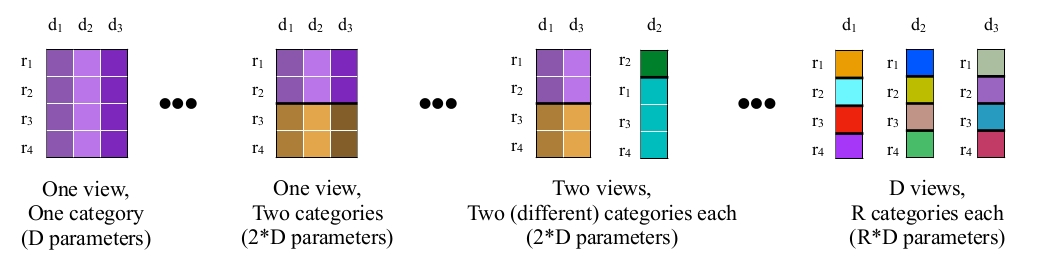
\includegraphics[width=0.8\textwidth]{cc.jpeg}
\caption{Some possible cross-categorizations of a table with 3 columns
  and 4 rows.  Any two cells with different colors are taken to be
  independent conditioned on the latent structure.}
\label{fig:cc}
\end{figure}
The collection of all possible column/row partitions $j$ of
$\mathbf{X}$, with their associated component parameters $\theta$,
defines a GPM class:

$\mathcal{M}_\textbf{X} = \set{CC_j^{\theta} \text{ : cross-cat of } \mathbf{X}
\text{ with partition } j \text{ and component model params } \theta}$.

A member of the CrossCat GPM class is a particular
cross- categorization with partition $j$ and component parameters
$CC_j^{\theta^*}$.  Adding a prior over these possible structures
defines an adaptive generative population model.
\end{example}

Unlike Example~\ref{ex:normal_gpm}, the latent information of the GPM
in Example~\ref{ex:crosscat} is structurally dependent on
the statistical population it has produced $\mathbf{X}$. Observing more
generated members $\mathbf{X} \to
\mathbf{X}'$ means the GPM class under consideration grows from
$\mathcal{M}_\textbf{X}$ to $\mathcal{M}_\textbf{X'}$, as both the number of
possible cross-categorizations $j$ and the dimensionality of the vector of
latents $\theta$ increase.

\todo[inline]{The reason I am being so pedantic about this construction is to
explicate various design choices when simulating, sampling, and running
posterior inference. In particular we are going to have to break down the latent
structure into 'global' vs 'row-related' latents to differentiate between
observed and hypothetical members.}

The default adaptive GPM is not obliged to model all columns jointly by
positing some GPM from the CrossCat class. The MML includes modeling
instructions for describing dependence constraints, and specifying a
compositional, directed-acyclic network of arbitrary GPMs implemented by a user.
It also includes inference instructions for initializing adaptive GPMs and
performing updates of the posterior distribution on GPMs.

The MML is thus a complete (but sub-Turing) probabilistic programming language
that interoperates with queries written in BQL. The set of primitive GPMs can be
extended by loading foreign GPMs written in VentureScript or Python, and can be used to
transparently integrate models from disparate probabilistic programming
languages such as Stan and statistical computing environments such as R. Because
BQL programs only depend on the statistical data types of the columns, the
underlying modeling technologies, GPM assumptions, and inference tactics can be
changed without invalidating end-user data analysis workflows.

\section{Interface for Generative Population Models} \label{sec:generators}
A \textit{generative population model} is a probabilistic model of a data
generating process and a statistical population that it has produced. It is
informative to think of this statistical population as an infinite table
$\mathbf{X}$ with a finite number of columns $D$ (representing attributes) and
an infinite number of rows (representing members of the population). A finite
number of rows $r_i \in
\set{1,\dots,N}$ are actually observed, so $\mathbf{X}$ is stored in BayesDB as
an $N \times D$ table. Hypothetical members may be referenced by any other row index,
for example by drawing a random real row index
$r^*\sim U[0,1]$.

\begin{discussion} \label{disc:iid} Technical Aside On IID Rows

The classical statistical framework generally assumes that all members of a
population are independent and identically distributed. While a particular
generator is free to make any assumptions about its population, the IID
assumption is a strong one. The default generator (and almost any generator
being learned under the Bayesian framework) will usually assume that the rows
are not IID but exchangeably coupled. De Finetti's theorem guarantees that there
exists a mixture of random measures $\set{\G_\alpha}$ (which in most
cases is indexed by the latent state of the GPM) where the population is
conditionally IID.

$$p(\mathbf{X}) = \int_\alpha{(\Pi_{i=1}^Np(\mathbf{X}_i|\G_\alpha))d
\mathcal{Q}(\G_\alpha)}$$

The De Finetti measure $\mathcal{Q}$ is the object which defines a distribution
over the (fixed) measures (GPMs) that produce a statistical population. In this
sense, $\mathcal{Q}$ represents the adaptive GPM.

\end{discussion}

Generative population models provide the primitive statistical inferences that
are used by BayesDB to implement inferential queries in BQL. To support all of
BQL, a GPM must provide the ability to \textbf{sample from} and \textbf{evaluate
the log density of}\footnote{With respect to counting measure for variables of
discrete statistical types and Lebesgue measure for continuous.}
all possible marginal distributions subject to equality
constraints for arbitrary subsets of variables.

\subsection{Non-Adaptive GPMs}
\label{sec:non-adaptive_gpm}

Since non-adaptive GPMs are by assumption IID on the individuals in
the population, they admit a simpler interface than adaptive ones.  As
such we present it first, and defer the generalization to
Section~\ref{sec:adaptive_gpm}.

\begin{enumerate}

\item \texttt{$\G$ = initialize(schema = $\Lambda$)}

    Initialize a GPM with the given schema, and return the resulting GPM
    $\G$.

    Each GPM is initialized with a \textit{schema} $\Lambda=$\path{(typed-
    outputs, typed-inputs, body)}. The \path{typed- outputs} component specifies
    the column indexes and statistical types of each column that the GPM will be
    responsible for generating. The \path {typed-inputs} component specifies the
    indexes and statistical types of columns that the GPM can read
    from.  If this set is non-empty, the GPM is \emph{conditional}.
    The \path{body} is a GPM-specific blob (opaque to BayesDB) that contains any
    desired configuration information.

\item \texttt{$\vec{s}$ =
    simulate($\G$, row = $i$, targets = $\set{c_j}_{j=1}^{|T|}$, givens
    = $\set{(c_k, x_{ik})}_{k=1}^{|G|}$)}

    Generate a sample from the specified conditional distribution on columns:
    $$
    \vec{s} \sim p( \set{ \mathbf{X}_{ij} } |
    \set{ \mathbf{X}_{ik} = x_{ik} }, \G).
    $$

    The returned $\vec{s}$ is a $|T|$ dimensional vector.

\item \texttt{$\log p$ =
    logpdf($\G$, row = $i$, targets = $\set{(c_j, x_{ij})}_{j=1}^{|T|}$,
    givens = $\set{(c_k, x_{ik})}_{k=1}^{|G|}$)}

    Evaluate the log probability density of the specified conditional
    distribution on columns at a target point:

    $$
    \log p = \log p( \set{ \mathbf{X}_{ij} = x_{ij} } |
    \set{ \mathbf{X}_{ik} = x_{ik} }, \G).
    $$

    The density is with respect to a product of counting and Lebesgue
    measures, correspoding to discrete and continuous statistical
    types for the relevant columns.  The distribution is interpreted
    as marginalizing out all random variables that are not mentioned.

\end{enumerate}

The column indexes $c_j, c_k$ referred to above must refer to columns
present in the table---the MML does not have a notion of hypothetical
columns.  Further, the \texttt{target} indexes must be a subset of the
columns in the \texttt{typed-outputs} of the GPM $\G$, and
the \texttt{given} indexes of each query must be a superset of the
\texttt{typed-inputs} of the GPM $\G$.  Note: A client may
specify some of the \texttt{typed-outputs} as \texttt{given} in any
given query.  Doing so picks out a conditional version of the output
distribution.

The row index $i$ may either refer to an individual in the
table, or a hypothetical individual.  In the former case, the
distribution being sampled or assessed is taken as conditional on
whatever latent information is available about that individual, but
\emph{not on any attributes stored in the table} except as repeated in
the \texttt{givens}.  In the latter case, the distribution is taken to
refer to a fresh individual (i.e., marginalizing out any
per-individual latent structure).

\subsection{Formalism for Adaptive GPMs}
\label{sec:formalism-adaptive-gpm}

As outlined in Section \ref{sec:overview}, some GPMs can be learned
from observations $\set{\mathbf{X}_{ij} = x_{ij}}$ of a statistical population
$\mathbf{X}$.  Since we permit the learning to itself be stochastic,
the general case is a family of conditional probability distributions
(of learning results) for all possible sets of observations.  Formally:

\begin{definition} Adaptive Generative Population Model

An \emph{Adaptive Generative Population Model} over a class of GPMs
$\{\G_\alpha\}$ is a family of conditional probability distributions
$\Pi(\G_\alpha|\{\mathbf{X}_{ij} = x_{ij}\})$, for all possible
observation sets $\{x_{ij}\}$.
\end{definition}

\todo[inline]{Figure out whether we want the Adaptive GPM to be defined as a 
family of  conditional distributions $\Pi\set{\mathcal{G}_\alpha}$ indexed by 
$\alpha$, or just define it as  $\Pi$, which is the distribution over the
$\mathcal{G}_\alpha$.}

\begin{example} Linear Regression

Linear regression (with a fixed noise model $\mathcal{E}$) can be viewed as a
conditional adaptive GPM over the class of non-adaptive GPMs
parameterized by the possible regression coefficients $\vec\beta_j$.
For input columns $\{x_j\}$ and output column $y$,
the update rule corresponding to maximum likelihood estimation would be

\[ \vec\beta_j^*|\{x_{ij}, y_i\} = \argmax_{\vec\beta_j^*} \sum_i 
p_{\mathcal{E}}(y_i - x_{ij}^T \beta_j^*). \]

The {\tt simulate} and {\tt logpdf} methods would refer to the
noise distribution around the predicted value for $y$.

\todo[inline]{Clear up this notation.
    How can $x_{ij}$, which is just a cell, have a vector operation?
    What is $j$ indexing?
    We seem to maximize the probability of the noise by subtracting the
    observation from the conditional mean. The more natural
    way to express the MLE is maximize the observation $y_i$ conditioned
    on the data, ie $p(y_i|x_i\beta)$. Although the noise model $\mathcal{E}$
    is fixed, we still do not know the parameters $\sigma$ of the noise,
    and that is typically learned from data as well.
    We are also overloading $\set{x_j}$ to mean columns, observations, etc.}
\end{example}

\begin{example} Exact Bayesian Adaptive GPMs

For any GPM class $\{\G_\alpha\}$, an \emph{exact Bayesian adaptive
  generative population model} is given by a prior
$\Pi(\G_\alpha)$ over
$\{\G_\alpha\}$, and the adaptation rule

\[ \Pi(\G_\alpha|\set{\mathbf{X}_{ij} = x_{ij}}) \propto \Pi(\G_\alpha)
 p(\set{\mathbf{X}_{ij} = x_{ij}}|\G_\alpha), \]

where $p(\cdot|\G_\alpha)$ is the probability of the observed data under
the particular GPM $\G_\alpha$. \label{ex:exact-bayes}

\todo[inline]{I killed the vector notation which I discourage from
    using, especially when coupling a vector with two subscripts and
    throwing it inside a set.
    I brought back the $\mathbf{X}$ the random 
    table, to keep it at the forefront. The table
    is essential to discussion of GPMs, and is a familiar notation.}
\end{example}

\subsection{Incremental Adaptive GPMs}

The desired adaptation rule of an adaptive GPM (such as the exact
Bayesian rule of Example~\ref{ex:exact-bayes}) may not always be
tractable to compute.  BayesDB permits adaptive GPMs to expose a
time-accuracy tradeoff in the form of incremental adaptation, where
the client is invited to select the amount of computational resources
they are willing to commit, and rewarded for greater commitment with a
superior quality of adaptation.  Formally this involves adding a ``fuel''
parameter to the adaptation rule:

\begin{definition} Incremental Adaptive Generative Population Model
\label{def:incremental-adaptive}

An \emph{Incremental Adaptive Generative Population Model} over a
class of GPMs $\{\G_\alpha\}$ is a family of conditional probability
distributions $\Pi_n(\G_\alpha|\set{\mathbf{X}_{ij} = x_{ij}})$, for all
possible observation sets $\{x_{ij}\}$ and all positive integers $n$,
where increasing $n$ represents increasing computational
cost.\footnote{In Section~\ref{sec:adaptive_gpm} we will specify a
  somewhat more flexible interface to learning than iterating a single
  transition operator, but spelling that out at this point would be
  needlessly notationally cumbersome.}
\end{definition}

\begin{example} Bayesian Markov Adaptive GPMs

For any GPM class $\{\G_\alpha\}$, a \emph{Bayesian Markov adaptive
  generative population model} is given by a prior
$\Pi(\G_\alpha)$ over
$\{\G_\alpha\}$, a data-dependent transition operator
$\T_{\{\vec{x}_{ij}\}}$ over $\{\G_\alpha\}$, and
an adaptation rule that consists of iterating $\T$:

\[ \Pi_n(\G_\alpha|\set{\mathbf{X}_{ij} = x_{ij}}) = \T_{\set{x_{ij}}}^n 
\Pi(\G_\alpha). \]
\label{ex:markov-bayes}
\end{example}

This will be \emph{asymptotically Bayesian} if the transition operator
converges to the true posterior, that is if

\[ \lim_{n\to\infty}D_{KL}(\Pi^*(\G_\alpha) \| \Pi_n(\G_\alpha|\{\vec{x}_{ij}\})) = 0, \]

where $\Pi^*(\G_\alpha|\set{\mathbf{X}_{ij}=x_{ij}}) \propto 
\Pi(\G_\alpha) p(\set{\mathbf{X}_{ij}=x_{ij}}|\G_\alpha)$
as in the exact Bayes case (Example~\ref{ex:exact-bayes}).
If the true data distribution falls into the hypothesis class given by
the prior $\Pi$, this will also be \emph{asymptotically consistent} in
the usual sense.

Since non-incremental adaptive GPMs are a special case of incremental
ones, we will make the assumption of incrementality in the rest of
this document, and omit the adjective.

\subsection{Interface for Adaptive GPMs}
\label{sec:adaptive_gpm}

The extended interface for adaptive GPMs based on Markov chains is outlined
below.  The key differences from the interface to non-adaptive GPMs
defined in Section~\ref{sec:non-adaptive_gpm} are as follows:

\begin{itemize}
\item We add \texttt{incorporate} and \texttt{remove} methods to
  manipulate the set of observed individuals on which the adaptive GPM
  is taken to be conditioned.
\item We add an \texttt{infer} method to control expenditure of
  computation on incremental adaptation.
\item We generalize the \texttt{simulate} and \texttt{logpdf} methods
  to permit querying and conditioning on multiple rows, since the
  joint distribution on several rows need no longer be the product of
  the corresponding marginal distributions.
\end{itemize}

Note: BayesDB implements an algorithm for recovering joint multi-row
simulation in terms of single-row simulations, so the multi-row
version of \texttt{simulate} may be viewed as an optional
optimization.

\todo[inline]{An adaptive GPM can be used as a non-adaptive GPM by
  marginalizing out the distribution over the class it is supposed to
  adapt over.  Technical difficulty: that calls for non-incorporating
  simulations, whereas the promised algorithm for multi-row simulate
  in terms of single-row simulate relies on simulations incorporating
  their results (which is expected to be cheap).}

\todo[inline]{Analogous issue with drawing multiple samples from block
  simulation.  The samples are supposed to be IID; which one does the
  simulation incorporate?}

\begin{enumerate}

\item \texttt{$\G$ = initialize(schema = $\Lambda$)}

    Initializes an adaptive GPM with the given schema \texttt{$\Lambda$ =
    (typed-outputs, typed-inputs, body)}.  This is identical with the
    \texttt{initialize} operation for non-adaptive GPMs.  The distribution $\Pi$
    on adaptations is taken to be conditioned on the empty set of observations
    $\Pi(\G_\alpha|\{\})$.
    
    \todo[inline]{I take it the last sentence is just a fancy way to say ``the 
    prior"?}

\item \texttt{$\vec{s}$ =
    simulate($\G$, targets = $\set{(r_j,c_j)}_{j=1}^{|T|}$, givens
    = $\set{(r_k, c_k, x_{r_kc_k})}_{k=1}^{|G|}$)}

    Generate a joint sample from the specified conditional
    distribution on cells.
    $$
    \vec{s} \sim p( \set{ \mathbf{X}_{r_jc_j} } |
    \set{ \mathbf{X}_{r_kc_k} = x_{r_kc_k} }, \G)
    $$

    Note that $\vec{s}$ is a $|T|$ dimensional vector of the simulated
    values for those cells.  As in the non-adaptive case
    (Section~\ref{sec:non-adaptive_gpm}), row indexes control conditioning
    or lack thereof on per-individual latent structure, but all conditioning
    on manifest structure is determined by the \texttt{givens}.
    
    \todo[inline]{This is as far as we have reached with the rewrite.}

\item \texttt{$\log p$ =
    logpdf($\G$, targets = $\set{(r_j, c_j, x_{r_jc_j})}_{j=1}^{|T|}$,
    givens = $\set{(r_k, c_k, x_{r_kc_k})}_{k=1}^{|G|}$)}

    Evaluate the log probability density of the specified conditional
    distribution on cells at a target point.

    $$
    \log p = p( \set{ \mathbf{X}_{r_jc_j} = x_{r_jc_j} } |
    \set{ \mathbf{X}_{r_kc_k} = x_{r_kc_k} }, \G)
    $$

    As in the non-adaptive case, the density is with respect to a
    product of counting and Lebesgue measures, correspoding to
    discrete and continuous statistical types for the relevant
    columns.  The distribution is interpreted as marginalizing out all
    random variables that are not mentioned.

\item \texttt{incorporate($\G$, value = $(i, j, x_{ij})$)}

    Record an observation $x_{ij}$ in the cell $\mathbf{X_{ij}}$.
    If there is no row $i$, create a new one.

    It is an error for the client to overwrite existing cells, or to insert values
    $x_{ij}$ incompatible with the schema $\Lambda$ (for example,
    providing data of the wrong type).

    Consecutive calls to \texttt{incorporate} (and \texttt{remove})
    should commute.  In the case of incremental GPMs, intervening
    \texttt{infer} is permitted to break commutativity.

\item \texttt{remove($\G$, $(i, j)$)}

    Remove the observation $x_{ij}$ stored in cell $\mathbf{X}_{ij}$.
    Consecutive \texttt{remove} should exactly invert
    \texttt{incorporate} on the same cell.  In the case of incremental
    GPMs, intervening \texttt{infer} is permitted to change the
    result.  (That is, \texttt{incorporate}, \texttt{infer}, \texttt{remove}
    may be different from just the \texttt{infer}.)

\item \texttt{infer($\G$, program = $\mathcal{P}$)}

    Adjust any internal latent state in accordance with the inference
    procedure specified in the program $\mathcal{P}$.  To BayesDB, the
    inference program is an opaque blob; the menu of accepted
    inference programs is expected to be designed in tandem with the
    \texttt{body} specified in the schema $\Lambda$.

    In the case where $\G$'s state is samples from the current state
    of a Markov chain, $\mathcal{P}$ would specify application of a
    transition operator.  If that operator were asymptotically
    Bayesian, each run of \texttt{infer} would improve the quality
    with which the distribution on sub-models $\{\G_\alpha\}$
    approximates the posterior.
\end{enumerate}

Note that the interface specified above is somewhat more flexible than
Definition~\ref{def:incremental-adaptive} given for incremental
adaptive GPMs.  In particular:

\begin{itemize}
\item Addition (and removal) of data may be interleaved with learning
  and querying.
\item A GPM may specify a menu of possible inference programs as
  options for learning, in which case the learned distribution on
  $\{\G_\alpha\}$ would depend on the sequence of arguments passed to invocations
  of \texttt{infer} (and how they are interspersed with
  \texttt{incorporate} and \texttt{remove}), rather than simply on
  their count as Definition~\ref{def:incremental-adaptive} suggests.
\end{itemize}

\subsection{Ensembling Adaptive GPMs}
\label{sec:ensemble}

If BayesDB inferences were based on a single instance of an adaptive
GPM, the inferences could arbitrarily suppress modeling
uncertainty. The MML provides users a generic \emph{GPM ensemble}
mechanism, that can be used for measuring and improving accuracy of
inferences.  In the language of Markov Chains, the ensemble represents
a set of independent, parallel chains, which answers queries by simple
Monte Carlo over its constituents.

An ensemble of (adaptive, incremental) GPMs is itself an (adaptive,
resp.\ incremental) GPM.  The default ensemble implements the GPM interface of
Section~\ref{sec:adaptive_gpm}
interface as follows:

\begin{enumerate}
\item \texttt{$\mathcal{Q}$ = initialize(schema = $\Lambda$, count = S)}

    Accepts an additional \texttt{count} argument, to specify the size
    of the ensemble.  Operationally, initializes a collection of $S$
    GPMs with the schema $\Lambda$ (independently, if the
    initialization is stochastic).
    $$
    \mathcal{Q} = (\set{\G_s}_{s=1}^S, \mathbf{X_\mathcal{Q}})
    $$

    The schema and data store are shared across all GPMs in the
    ensemble.

\item \texttt{simulate} delegates to a uniformly random ensemble
  element $\G_k$.

    $$
    \vec{s} = \texttt{simulate} (\G_*,\dots) \text{ where }
    \G_* \sim U[\set{\G_s}]
    $$

  \todo[inline]{Maybe conditional simulation should weight the ensemble
    elements by how likely those conditions are in them?  It can, by
    invoking their logpdf methods.  This would worsen the asymptotic
    complexity of simulate, though.}

\item \texttt{logpdf} forms a Monte Carlo estimate of the expected density using
all of the GPMs in the ensemble.

    $$
    \log p = \logsumexp_s\texttt{logpdf}(\G_s) - \log S
    $$

\item \texttt{incorporate}, \texttt{remove}, and \texttt{infer} apply
  pointwise to all the GPMs in the ensemble.

\end{enumerate}

More elaborate methods such as likelihood weighting or particle
filtering ensembles are possible extensions.

\section{Derived Functions}

The operations \texttt{simulate} and \texttt{logpdf} are directly
accessible to BQL programs via the \texttt{SIMULATE} and
\texttt{PROBABILITY OF} syntax.  Other query functions may be
implemented generically in terms of \texttt{simulate} and
\texttt{logpdf}; though many of them may also have more efficient
short-cut implementations that are specific to the structure of a
given GPM.  This section lists the derived functions, their
definitions, and default implementations provided by BayesDB.

\todo[inline]{What time/accuracy knobs should be exposed in the
  interfaces?}

\subsection{Conditional Mutual Information}

\begin{definition} Conditional Mutual Information \todo{standard reference}

The \emph{conditional mutual information} (CMI) of two random variables $A$
and $B$ with respect to a third variable $C$ is the expectation, with
respect to $C$, of the mutual information of the conditional variables
$A|C$ and $B|C$.  In the discrete case this can be written as

    \begin{eqnarray*}
    I(A;B|C) & := &
        \sum_c p_C(c) \sum_{a,b} p_{A,B|C}(a,b|c) \log
            \frac{p_{A,B|C}(a,b|c)}{p_{A|C}(a|c) p_{B|C}(b|c)} \\
    &=& \sum_{a,b,c} p_{A,B,C}(a,b,c) \log
            \frac{p_C(c) p_{A,B,C}(a,b,c)}{p_{A,C}(a,c) p_{B,C}(b,c)}.
    \end{eqnarray*}

\end{definition}

In the context of the (notionally) infinite random table $\mathbf{X}$
induced by any given GPM $\G$,
BayesDB can estimate the joint conditional mutual information for any
three collections of cells $A$, $B$, $C$, itself in a population distribution
conditioned on given values $d$ for any fourth collection of cells $D$:

    \begin{align*}
    \set{(\hat{a}_j,\hat{b}_j,\hat{c}_j)}_{j=1}^n & \sim n \textrm{ iid samples from } p_{A,B,C|D=d} \\
    I(A;B|C,D=d) & \approx
        \sum_{\hat{a}_j,\hat{b}_j,\hat{c}_j} \log
         \frac{p_{C|D=d}(\hat{c}_j)
         p_{A,B,C|D=d}(\hat{a}_j,\hat{b}_j,\hat{c}_j)}
         {p_{A,C|D=d}(\hat{a}_j,\hat{c}_j) p_{B,C|D=d}(\hat{b}_j,\hat{c}_j)}
    \end{align*}

    The samples and log densities are computed by invoking
    \begin{align*}
    {\tt simulate}&(\G, {\tt targets} = A \cup B \cup C, {\tt givens} = (D, d)) \\
    {\tt logpdf}&(\G, {\tt targets} = C, {\tt givens} = (D, d)) \\
    {\tt logpdf}&(\G, {\tt targets} = A \cup C, {\tt givens} = (D, d)) \\
    {\tt logpdf}&(\G, {\tt targets} = B \cup C, {\tt givens} = (D, d)) \\
    {\tt logpdf}&(\G, {\tt targets} = A \cup B \cup C, {\tt givens} = (D, d))
    \end{align*}
    in the appropriate pattern.

\todo[inline]{Specify effort throttles and characterization of
  uncertainty (e.g., returning the entire set of $n$ point estimates)}
\todo[inline]{With an ensemble, there is a choice of whether to
  internally average the individual members' assessments, or to expose
  all of them for further uncertainty characterization (in any of
  several possible configurations)}

\begin{example} Mutual Information

The per-column mutual information available in BQL with the
\texttt{MUTUAL INFORMATION} syntax is a special case of CMI with
$C = D = \emptyset$ and $A = \set{*, c_1}$, $B = \set{*, c_2}$
singleton collections of cells of (the same) fresh individual's
attributes corresponding to the desired columns.
\end{example}

\subsection{Marginal Dependence Probability}

 $p = \texttt{marginal-dependence-prob}(\G,
    \texttt{colA}=c_i,
    \texttt{colB}=c_j,
    \texttt{accuracy}=N)$

    \todo[inline]{Figure out how to allow the user to set a throttle for desired
        accuracy. Here I am using a generic accuracy term both in marginal-
        depprob and CMI}

    Computes the probability, under the random latent structure of the GPM,
    that the two variables $\mathbf{X}_{r^*,c_i}$ and $\mathbf{X}_{r^*,c_j}$ are
    unconditionally independent.

    \begin{align*}
    \mathbb{P}_\G\set{I(\mathbf{X}_{r^*,c_i} : \mathbf{X}_{r^*,c_j} = 0)}
    \end{align*}

    Given that mutual information is zero if and only the two variables are
    statistically independent, the following simple Monte Carlo procedure is a
    suggested implementation.

    \begin{algorithm} \label{alg:marginal_depprob} First obtain a set of mutual
        information estimates by invoking {\tt CMI}

        \begin{align*}
        \set{I_k} = {\tt CMI}(
        \G,
        A = \set{(r_i^*,c_i)}, B = \set{(r_i^*,c_j)}, C = \emptyset, D =
        \emptyset,\\ {\tt accuracy} = N, {\tt size} = N)
        \end{align*}

        Return the fraction of samples from $\set{I_k}$ for which the mutual
        information is zero
        \begin{align*}
            p = \frac{1}{|\set{I_k}|}\sum_{k}{\mathbb{I}_{\set{0}}(I_k)}
        \end{align*}
    \end{algorithm}

\subsection{Marginal Dependence Magnitue}

 $r^2 = \texttt{marginal-dependence-magnitude}(\G,
    \texttt{colA}=c_i,
    \texttt{colB}=c_j,
    \texttt{accuracy}=N)$

    Computes an informational measure of correlation between
    $\mathbf{X}_{r^*,c_i}$ and $\mathbf{X}_{r^*,c_j}$ based on EH Linfoot. The
    implementation is straightforward.

    \begin{algorithm} \label{alg:linfoot} Compute a point estimate for the
        mutual information $I_0$ between $\mathbf{X}_{r^*,c_i}$ and
        $\mathbf{X}_{r^*,c_j}$ using an appropriate invocation of {\tt CMI}.

        Return the Linfoot measure $r^2$

        \begin{align*}
        r^2 = \sqrt{1 - \exp{(-2I_0)}}
        \end{align*}

    \end{algorithm}

    \todo[inline]{Should this function return a point estimate or a collection
    of estimates?}
    \todo[inline]{The Linfoot measure\\
        http://www.sciencedirect.com/science/article/pii/S001999585790116X\\ is
        what has been traditionally used by Bax. Linfoot is normalized between
        [0,1] but there are some questionable properties, if $Y=g(X)$ Linfoot is
        not guaranteed to be 1 (easy to construct example in discrete case).
        Moreover feedback from PPAML is that the zmatrices it produces are
        sparse and uninsightful, and give the implication that continuous
        variables are more dependent than categorical ones.}

\subsection{Generative Similarity}

  $r^2 = \texttt{generative-similarity}(\G,
    \texttt{context-vars} = \set{c_i},
    \texttt{rowA}=r_i,
    \texttt{rowB}=r_j,
    \texttt{accuracy}=N)$

    Computes the context-sensitive generative similarity for two members of the
    statistical population. This is defined as the probability, under the random
    latent structure of the GPM, that
    \texttt{rowA} and \texttt{rowB} are identically distributed conditioned on
    \texttt{context-vars}.

\subsection{Imputation}

\subsection{Correlation}

\subsection{Typicality}

\subsection{Column Similarity}

\section{TODOs}

    \todo[inline]{Explain what it means to have 'observed members' of a
    statistical population. In particular, a GPM's latentness can be broken down
    into 'global' and 'row-specific'. Specifying a row index is and implicit
    conditioning any distribution on the row-latents. This idea is mostly
    applicable to GPMs which implicitly cluster the observed population, (and
    carry a distribution over cluster assignments).}

\end{document}
